\documentclass[13spt]{beamer}

%packages
\usepackage[utf8]{inputenc}
\usepackage{amsmath}
\usepackage{amsfonts}
\usepackage{amssymb}
\usepackage{graphicx}
\usepackage{caption}
\usepackage{booktabs}
\usepackage[vietnamese]{babel}
\usepackage[orientation=landscape,size=custom,width=16,height=9,scale=0.5,debug]{beamerposter}
\usepackage{textpos}

%use
\usetheme{AnnArbor}
\definecolor{ballblue}{rgb}{0.13, 0.67, 0.8}
\definecolor{azure(colorwheel)}{rgb}{0.0, 0.5, 1.0}
\definecolor{blue(ryb)}{rgb}{0.01, 0.28, 1.0}
\definecolor{phthaloblue}{rgb}{0.0, 0.06, 0.54}
\usecolortheme[named =phthaloblue]{structure}
\usefonttheme{structurebold}
%---------------------------------------------------------------------------------------------------------------------------------------------------------
%begin
\begin{document}
\addtobeamertemplate{frametitle}{}{%
\begin{textblock*}{100mm}(.85\textwidth,-1cm)

\includegraphics[height=1cm,width=2cm]{logo.png}
\end{textblock*}}
\frametitle{TDP}
%\title{Bảo vệ khóa luận: \linebreak TÌM HIỂU VÀ VẬN DỤNG PHƯƠNG PHÁP XỬ LÝ DỮ LIỆU LỚN} {\color{black}\bfseries\inserttitle\par\vskip-6pt\hrulefill}

\title{Bảo vệ khóa luận: \linebreak TÌM HIỂU VÀ VẬN DỤNG PHƯƠNG PHÁP \hspace{5mm}XỬ LÝ DỮ LIỆU LỚN}
%\institute {Đại học thông tin liên lạc \linebreak Khoa công nghệ thông tin}


\author[ Trịnh Đình Phúc]{
\includegraphics[height=1.5cm,width=2.8cm]{logo.png} \\  \hspace{7mm} GVHD \hspace{6mm}: Th.S Cao Mạnh Hùng\\[3mm]{Sinh Viên : Trịnh Đình Phúc\\ \hspace{18mm}}}  

\date{\today} 
\frame{\titlepage} 

%page number
\setbeamertemplate{sidebar right}{}
\setbeamertemplate{footline}{%
\hfill\usebeamertemplate***{navigation symbols}
\hspace{1cm}\insertframenumber{}/\inserttotalframenumber}
\newcommand{\argmax}{\arg\!\max}

\frame{\frametitle{Nội dung báo cáo} \transblindshorizontal
\tableofcontents} 


\section{Giới thiệu} 
\subsection{Dữ liệu lớn}

\begin{frame}{Dữ liệu lớn là gì?}
\transblindshorizontal
  \begin{center}
    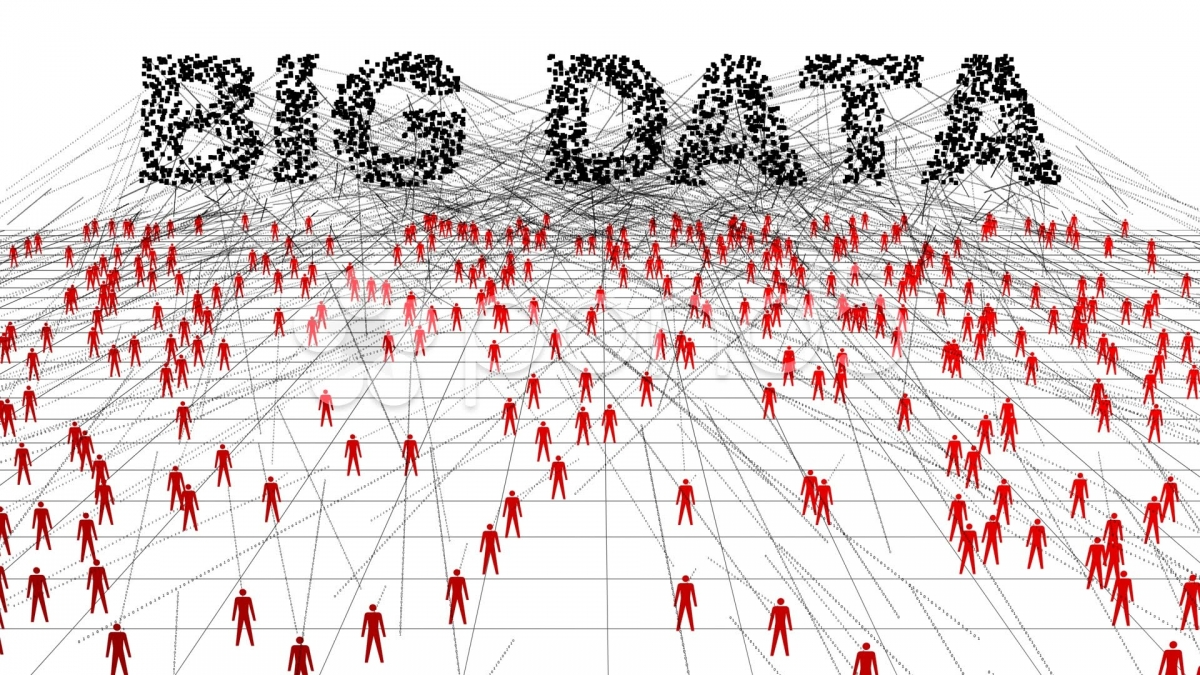
\includegraphics[width=1\linewidth,height=0.8\textheight,keepaspectratio]{big_data_robusta.jpg}
  \end{center}
\end{frame}

\begin{frame}{Dữ liệu lớn}
\transboxin
\textbf{Thống kê:} \pause
  \begin{center}
	\begin{itemize}
		\item 25+ TB dữ liệu được tạo ra mỗi giây trên toàn cầu.  \pause 
		\item 90+ \% dữ liệu của thế giới được tạo ra trong 2 năm vừa qua. \pause
		\item 90+ \% dữ liệu được tạo ra là dữ liệu phi cấu trúc.  \linebreak  \linebreak  \linebreak  \linebreak  \linebreak  \linebreak
    \end{itemize}
  \end{center}
\end{frame}
\transblindshorizontal
\begin{frame}{Các dạng dữ liệu lớn}
	\textbf{Dữ liệu có ở các dạng sau:}
\transboxin

\begin{center}
	\begin{tabular} {l l }
    \toprule
    \it Kiểu dữ liệu & \it Ứng dụng trong việc khai thác \\
    \midrule
    Văn bản & Xử lý ngôn ngữ tự nhiên  \\
    Ảnh và Video & Thị giác máy tính  \\  
    Âm thanh & Xử lý tín hiệu số  \\
    Social Network & Phân tích đồ thị  \\  
    Business & Khai thác dữ liệu  \\
    DNA & Tin sinh học \\           
    ... & ...\\            
    \bottomrule
    \end{tabular}
\end{center}

\end{frame}

\subsection{Làm thế nào để khai thác dữ liệu lớn?}
\begin{frame}{Làm thế nào để khai thác dữ liệu lớn?}
\transblindshorizontal

	\begin{figure}[h!]
	  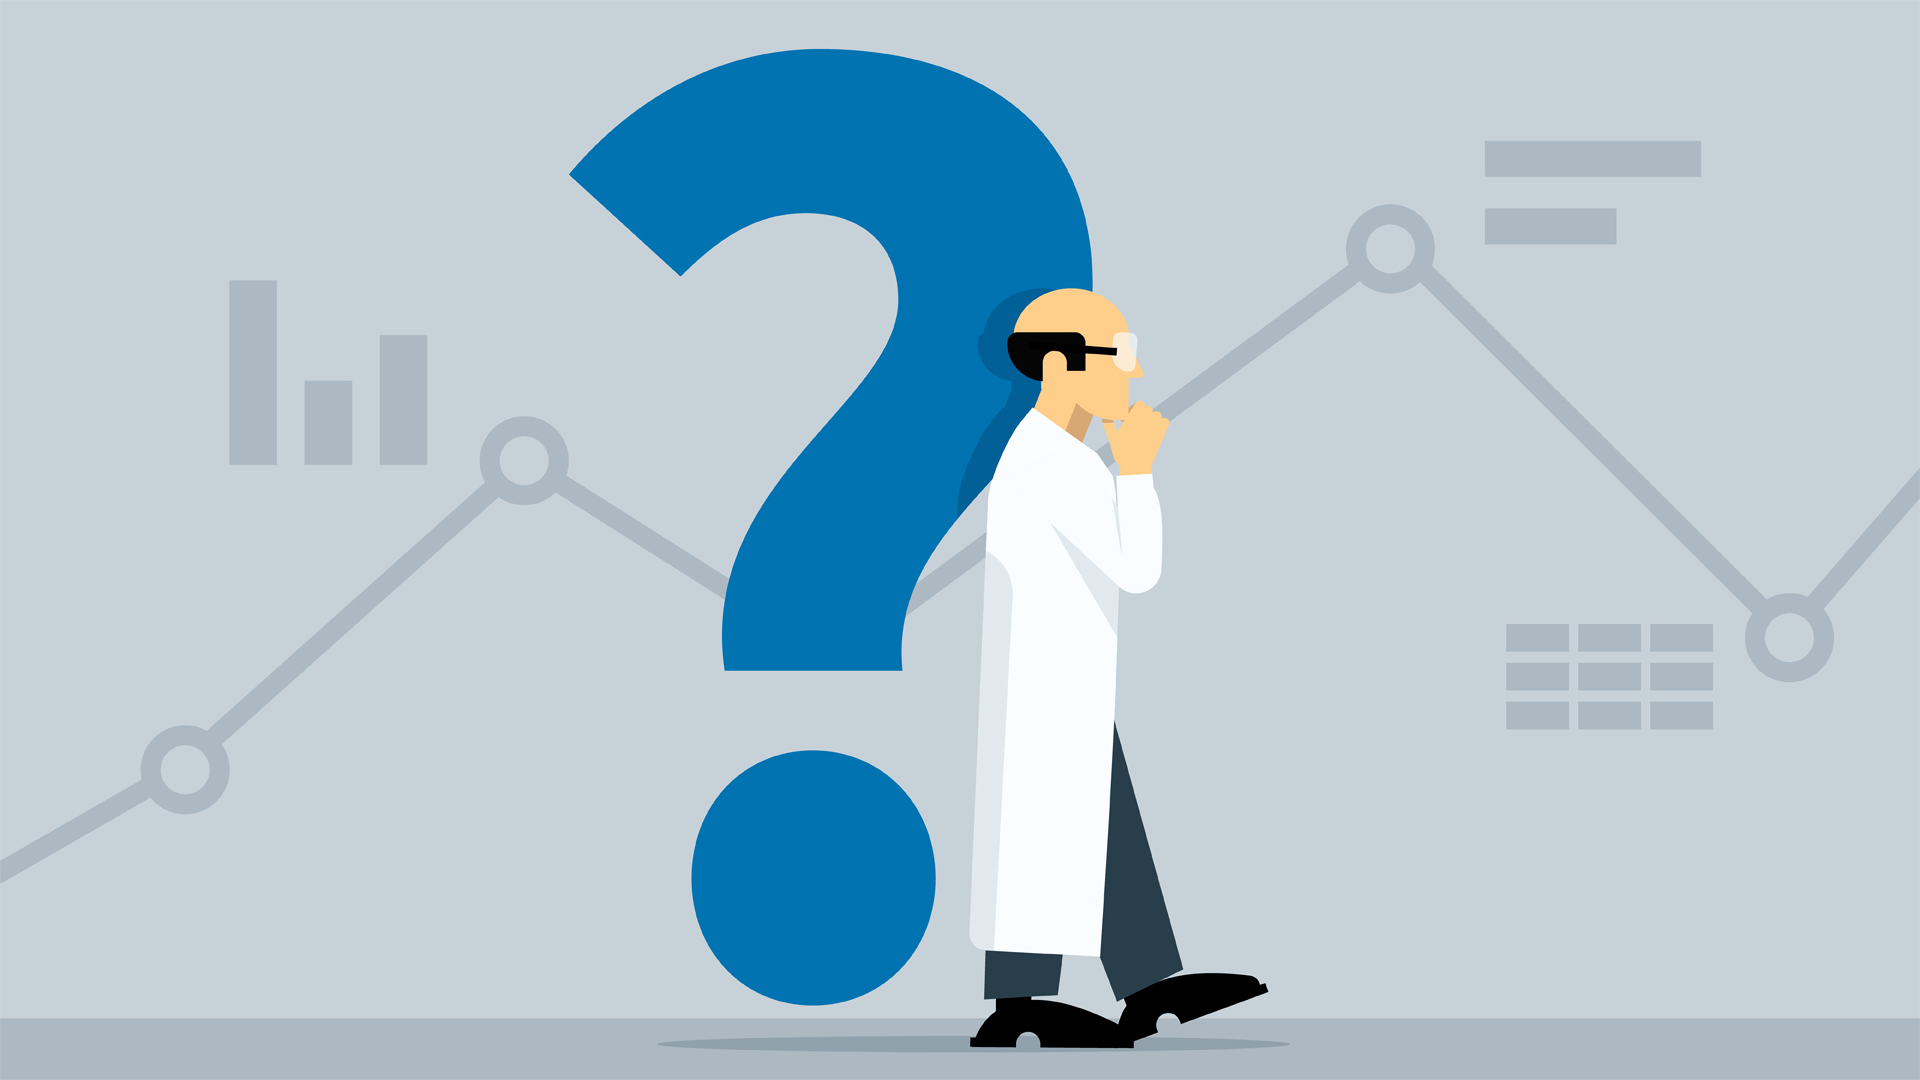
\includegraphics[width=1\linewidth,height=0.8\textheight,keepaspectratio]{why.jpg}
	  %\caption{Làm sao để khai thác "Dữ liệu lớn"?}
	  \label{fig:writing-thesis}
	\end{figure}
\end{frame}


\begin{frame}{Làm thế nào để khai thác Dữ liệu lớn?}
\transboxin

	\begin{figure}[h!]
	  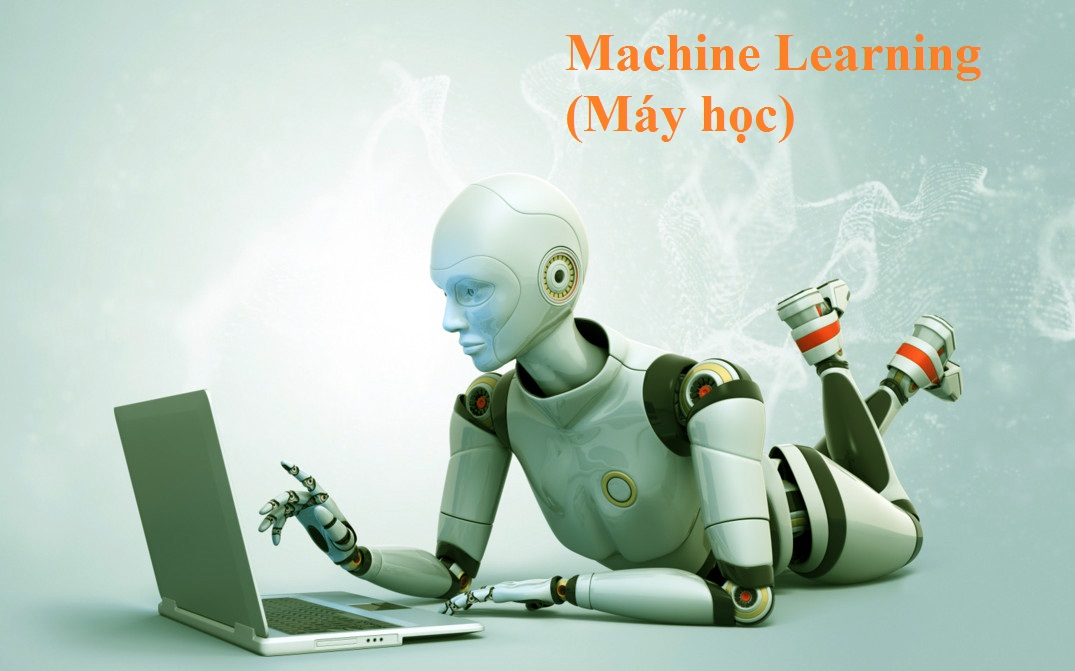
\includegraphics[width=1\linewidth,height=0.8\textheight,keepaspectratio]{machine-learning.jpg}
	  %\caption{Máy học}
	  \label{fig:writing-thesis}
	\end{figure}
\end{frame}

\section{Các bước khai thác dữ liệu}
\begin{frame}{Các bước khai thác dữ liệu}
\transblindshorizontal

 \begin{columns}
 \begin{column}{0.5\textwidth}
	\begin{figure}[h!]
	  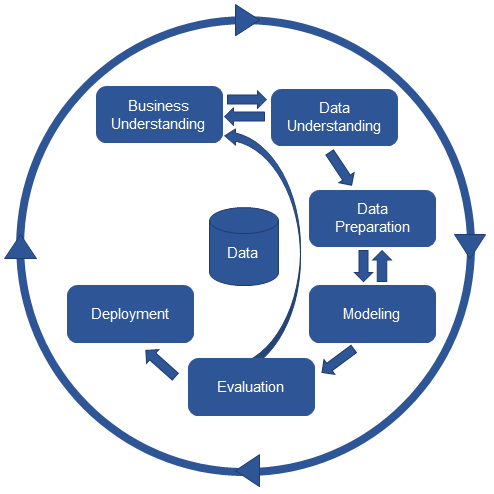
\includegraphics[width=1.2\linewidth,height=0.8\textheight,keepaspectratio]{CRISP-DM1.png}
	  %\caption{Quy trình khai thác dữ liệu CRISP-DM (Cross Industry Standard Process for Data Mining)}
	  \label{fig:writing-thesis}
	\end{figure}
 \end{column}
  \begin{column}{0.5\textwidth}
  \begin{small}

	\textbf{Quy trình khai thác dữ liệu có 6 bước chính: \small} \pause 

	\begin{enumerate}
	\item Tìm hiểu nghiệp vụ (Business understanding) \pause 
	\item Tìm hiểu dữ liệu (Data understanding) \pause 
	\item Chuẩn bị dữ liệu (Data preparation) \pause 
	\item Mô hình hoá (Modeling)
%		\begin{itemize}
%		\item Input: Dữ liệu
%		\item Output: Dự đoán tương lai, phân loại khách hàng, phát hiện hành vi giả mạo,... \pause
%		\end{itemize}
	\item Đánh giá mô hình (Model Evaluation)\pause 
	\item Triển khai (Deployment) 
	\end{enumerate}	
	\end{small}

 \end{column}
 \end{columns}
\end{frame}

\subsection{Thu thập dữ liệu (Data collection)}
\frame{\frametitle{Thu thập dữ liệu từ FIFA}
\transblindshorizontal
	\begin{figure}[h!]
	  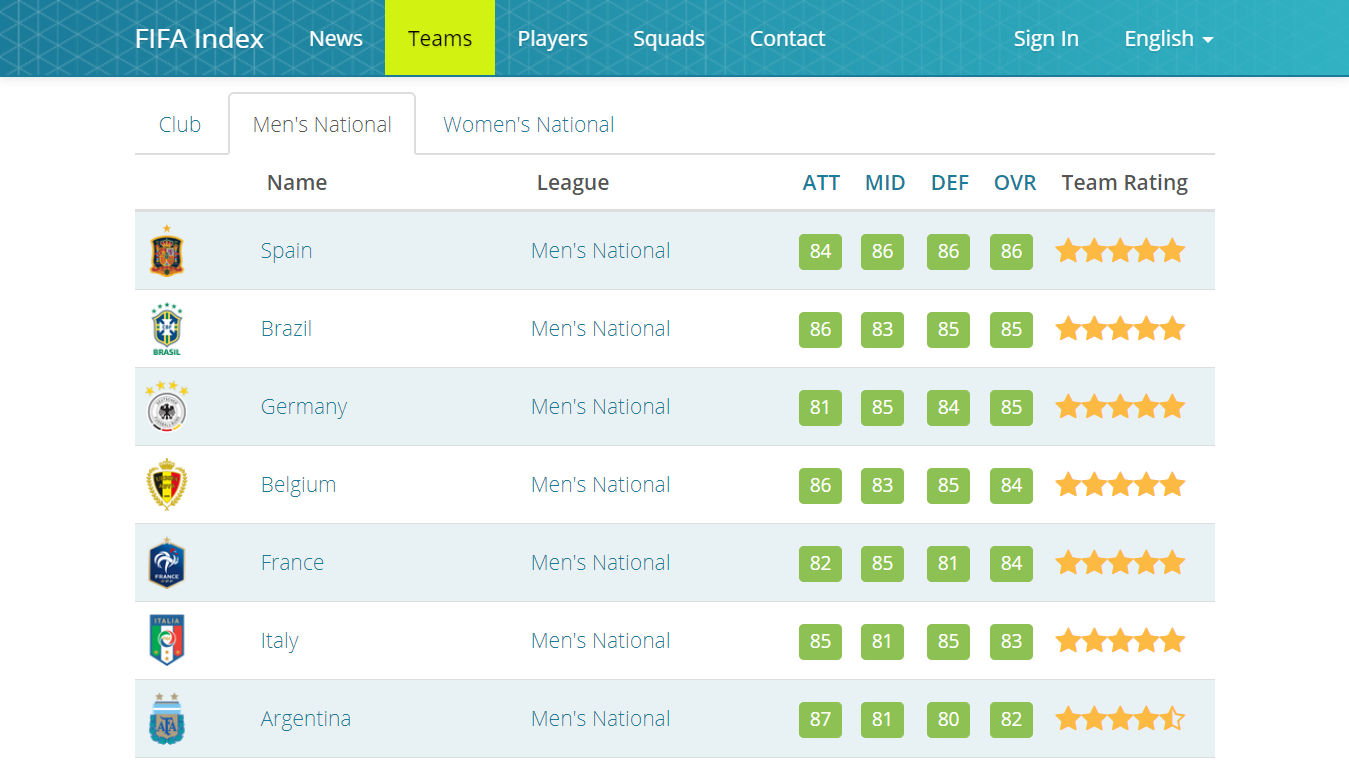
\includegraphics[width=1\linewidth,height=0.8\textheight,keepaspectratio]{fifa.png}
	  %\caption{Dữ liệu từ liên đoàn bóng đá thế giới FIFA}
	  \label{fig:writing-thesis}
	\end{figure}
}

\frame{\frametitle{Thu thập dữ liệu từ Mendeley}
\transblindshorizontal
	\begin{figure}[h!]
	  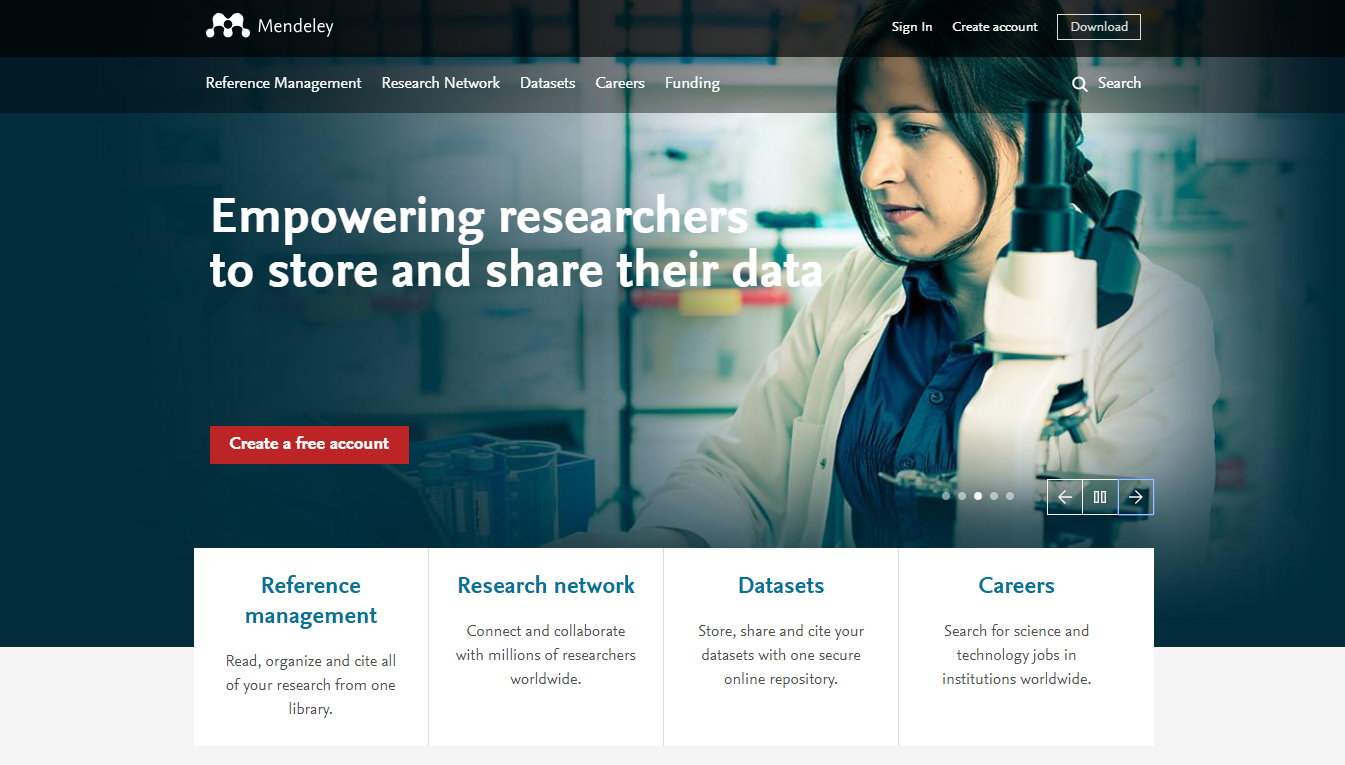
\includegraphics[width=1\linewidth,height=0.8\textheight,keepaspectratio]{X-Ray.png}
	   %\caption{Dữ liệu từ mạng xã hội học thuật tổ chức nghiên cứu, cộng tác Mendeley}
	  \label{fig:writing-thesis}
	\end{figure}
}

%\subsection{Tìm hiểu dữ liệu (Data understanding)}
%\frame{\frametitle{Tìm hiểu dữ liệu (Data understanding)}
%	\begin{figure}[h!]
%	  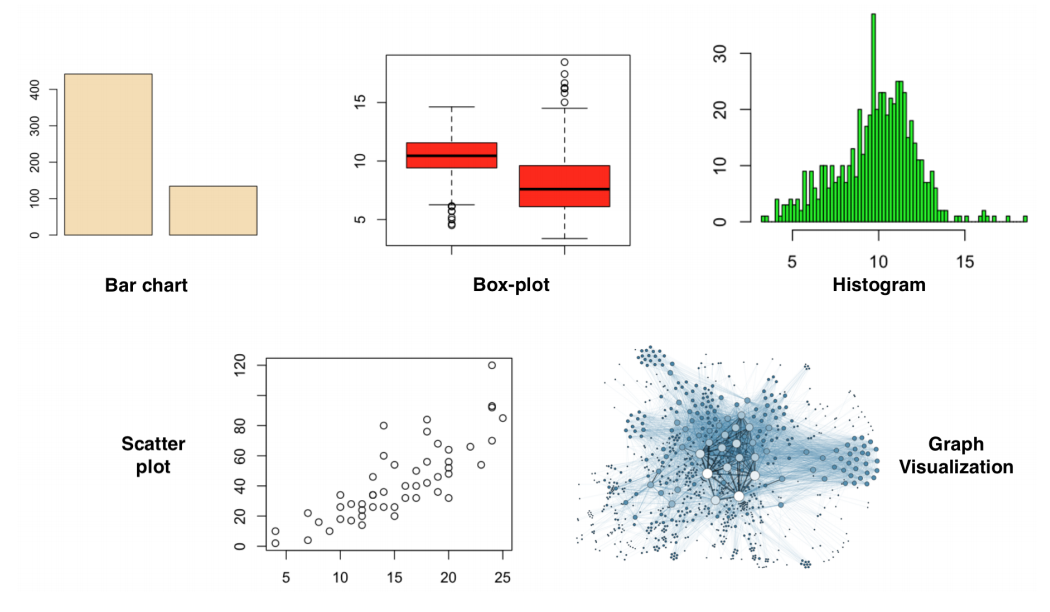
\includegraphics[width=1\linewidth,height=0.8\textheight,keepaspectratio]{plot.png}
%	  %\caption{Sử dụng các biểu đồ để phân tích}
%	  \label{fig:writing-thesis}
%	\end{figure}
%}
\subsection{Chuẩn bị dữ liệu (Data preparation)}
\frame{\frametitle{Chuẩn bị dữ liệu (Data preparation)}
\transblindshorizontal

 \begin{columns}
  \begin{column}{0.5\textwidth}
  \begin{small}

	\textbf{Các phương pháp tiền xử lý dữ liệu: \small}

	\begin{itemize}
		\item Bag of word
		\item TF-IDF
		\item Normalization
		\item PCA
		\item One-Hot-Encoding
		\item Feature Scaling
		\item Feature Selection
		\item Label Encoder
	\end{itemize} 
	\end{small}
 \end{column}
  \begin{column}{0.5\textwidth}
	\begin{figure}[h!]
	  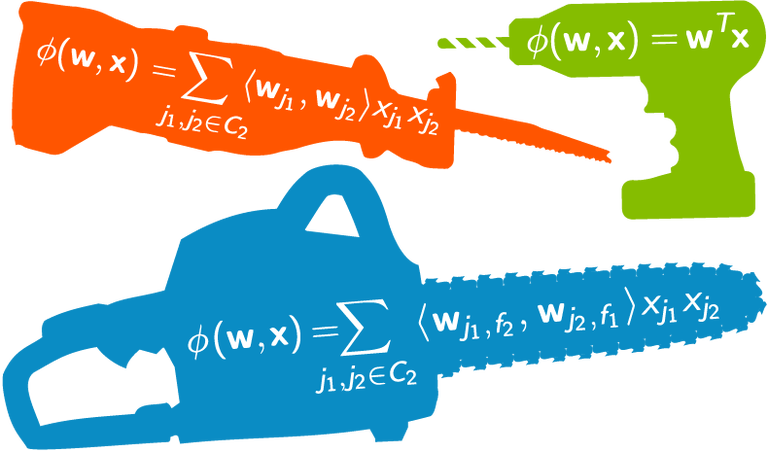
\includegraphics[width=1\linewidth,height=0.7\textheight,keepaspectratio]{feature-engineering.png}
	  \label{fig:writing-thesis}
	\end{figure}
 \end{column}
 \end{columns}

}

\subsection{Mô hình hoá (Modeling)}
\frame{\frametitle{Machine Learning - Học}
\transblindshorizontal
	\begin{figure}[h!]
	  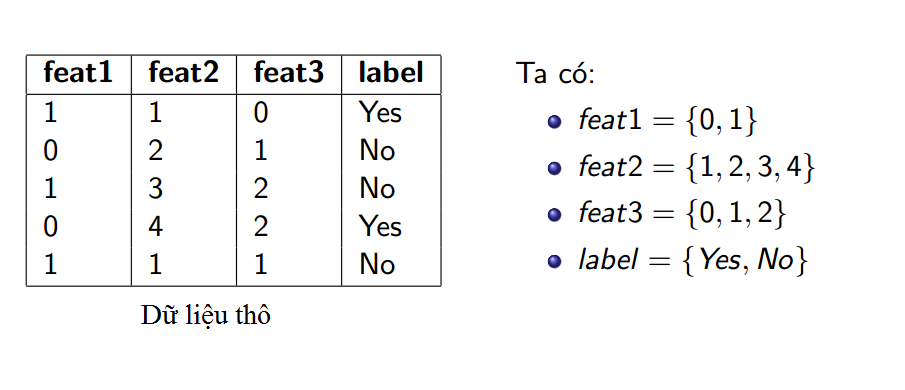
\includegraphics[width=0.9\linewidth,height=0.7\textheight,keepaspectratio]{modeling1.png}
	  \label{fig:writing-thesis}
	\end{figure}
}
\frame{\frametitle{Machine Learning - Dự đoán}
\transblindshorizontal
	\begin{figure}[h!]
	  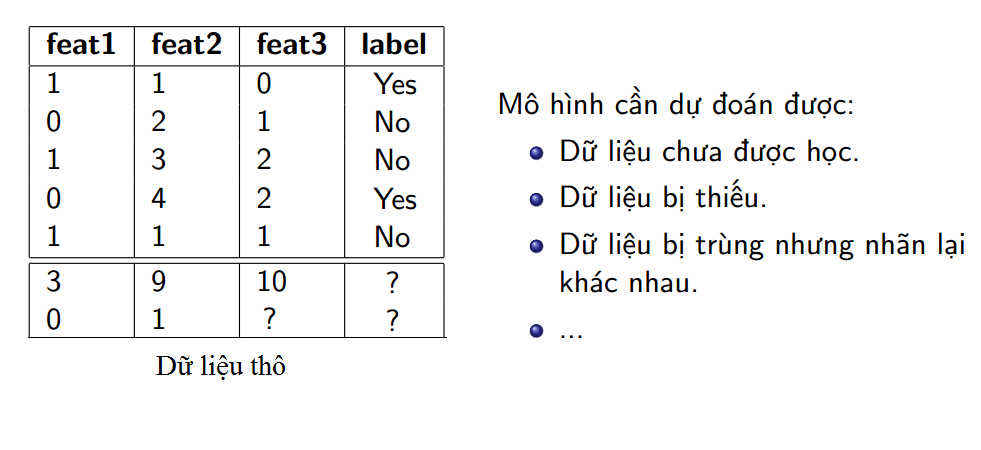
\includegraphics[width=0.9\linewidth,height=0.7\textheight,keepaspectratio]{modeling2.png}
	  \label{fig:writing-thesis}
	\end{figure}
}
\frame{\frametitle{Machine Learning - Dự đoán}
\transblindshorizontal
	\begin{figure}[h!]
	  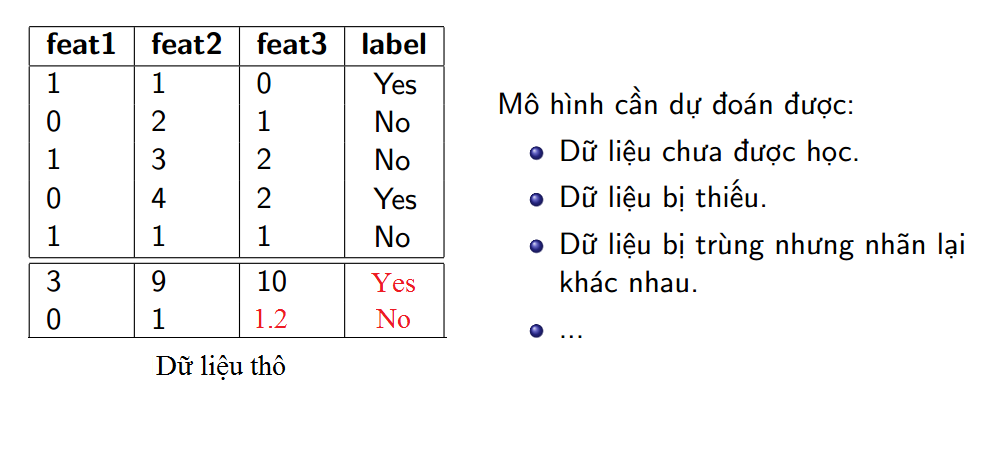
\includegraphics[width=0.9\linewidth,height=0.7\textheight,keepaspectratio]{modeling22.png}
	  \label{fig:writing-thesis}
	\end{figure}
}

\frame{\frametitle{Machine Learning - Thuật toán}
\transblindshorizontal
\begin{itemize}
\item Linear Regression/Ordinary least squares
	\begin{figure}[h!]
	  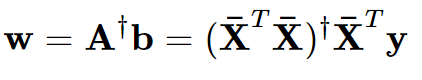
\includegraphics[width=0.3\linewidth,height=0.2\textheight,keepaspectratio]{linearregression.png}
	  \label{fig:writing-thesis}
	\end{figure}
\item Gradient Decent 
	\begin{figure}[h!]
	  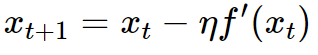
\includegraphics[width=0.25\linewidth,height=0.17\textheight,keepaspectratio]{gradientdecent.png}
	  \label{fig:writing-thesis}
	\end{figure}
\item Logistic Regression
	\begin{figure}[h!]
	  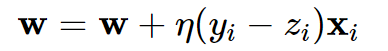
\includegraphics[width=0.3\linewidth,height=0.2\textheight,keepaspectratio]{logisticregression.png}
	  \label{fig:writing-thesis}
	\end{figure}
\item Support vector machine (SVM)
	\begin{figure}[h!]
	  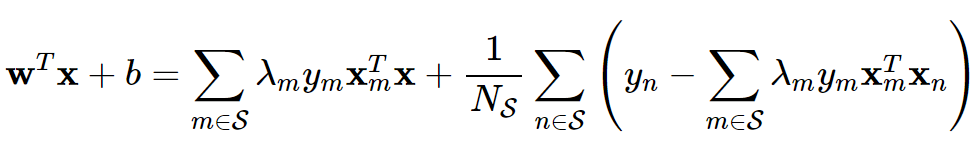
\includegraphics[width=0.58\linewidth,height=0.48\textheight,keepaspectratio]{svm.PNG}
	  \label{fig:writing-thesis}
	\end{figure}
\end{itemize}

}
\subsection{Đánh giá mô hình (Model Evaluation)}
\frame{\frametitle{Đánh giá mô hình}
\transblindshorizontal

 \begin{columns}
  \begin{column}{0.5\textwidth}
  \begin{small}
\begin{itemize}
\item Độ chính xác (Accuracy)
\item Ma trận nhầm lẫn (Confusion Matrix)  
\item True/False Positive/Negative
\item Receiver operating characteristic curve (ROC)
\item Area Under the Curve
\item Precision và Recall
\item Residual sum of squares (RSS)
\end{itemize} 
\end{small}
 \end{column}
  \begin{column}{0.5\textwidth}
	\begin{figure}[h!]
	  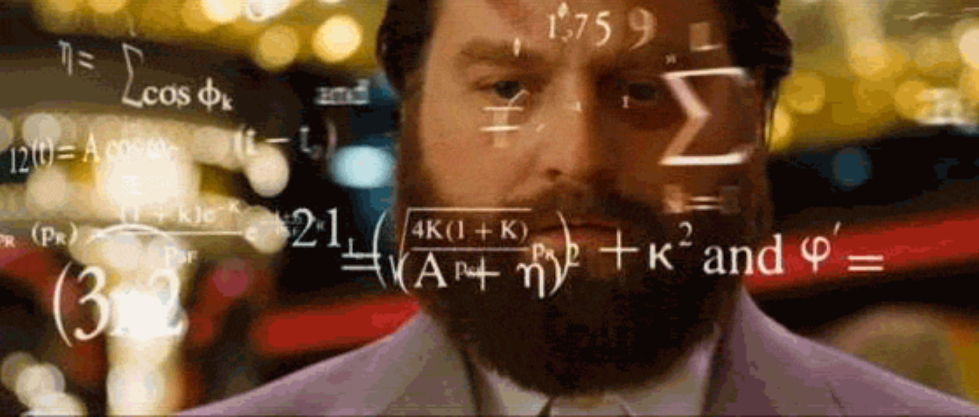
\includegraphics[width=1\linewidth,height=0.85\textheight,keepaspectratio]{hangover1.png}
	  \label{fig:writing-thesis}
	\end{figure}
 \end{column}
 \end{columns}
}

\section{Demo áp dụng quy trình xử lý dữ liệu lớn} 
\frame{\frametitle{Demo áp dụng quy trình xử lý dữ liệu lớn}
\transblindshorizontal

 \begin{columns}
  \begin{column}{0.5\textwidth}
	%\textbf{Các phương pháp tiền xử lý dữ liệu \small}
	\textbf{Dự đoán kết quả World Cup 2018 \linebreak(sử dụng máy học)\linebreak}
	\begin{figure}[h!]
	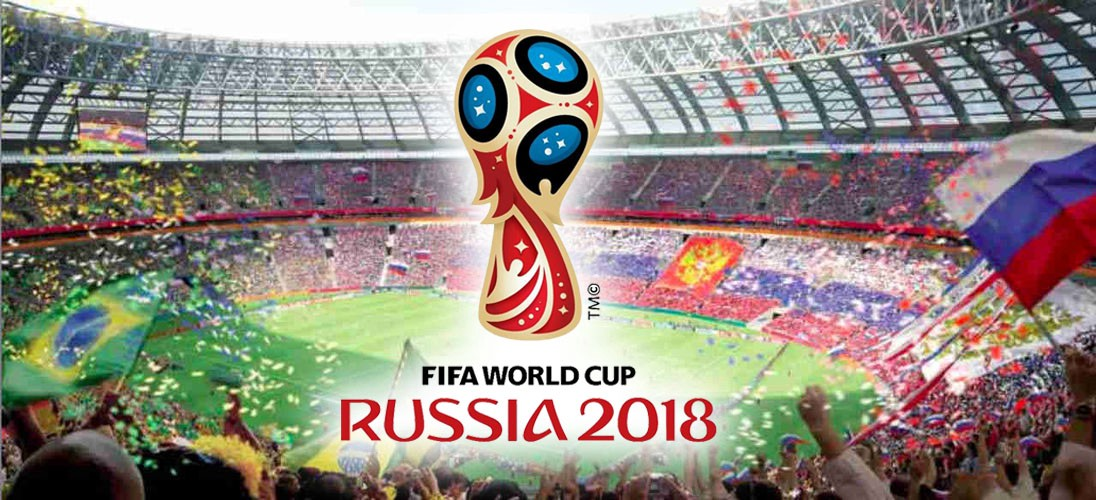
\includegraphics[width=1\linewidth,height=0.5\textheight]{show.jpeg}	  							\label{fig:writing-thesis}
	\end{figure}
 \end{column}
  \begin{column}{0.5\textwidth}
 	\textbf{Chuẩn đoán ung thư phổi qua ảnh X-quang (sử dụng mạng nơ-ron)\linebreak}
	\begin{figure}[h!]
 	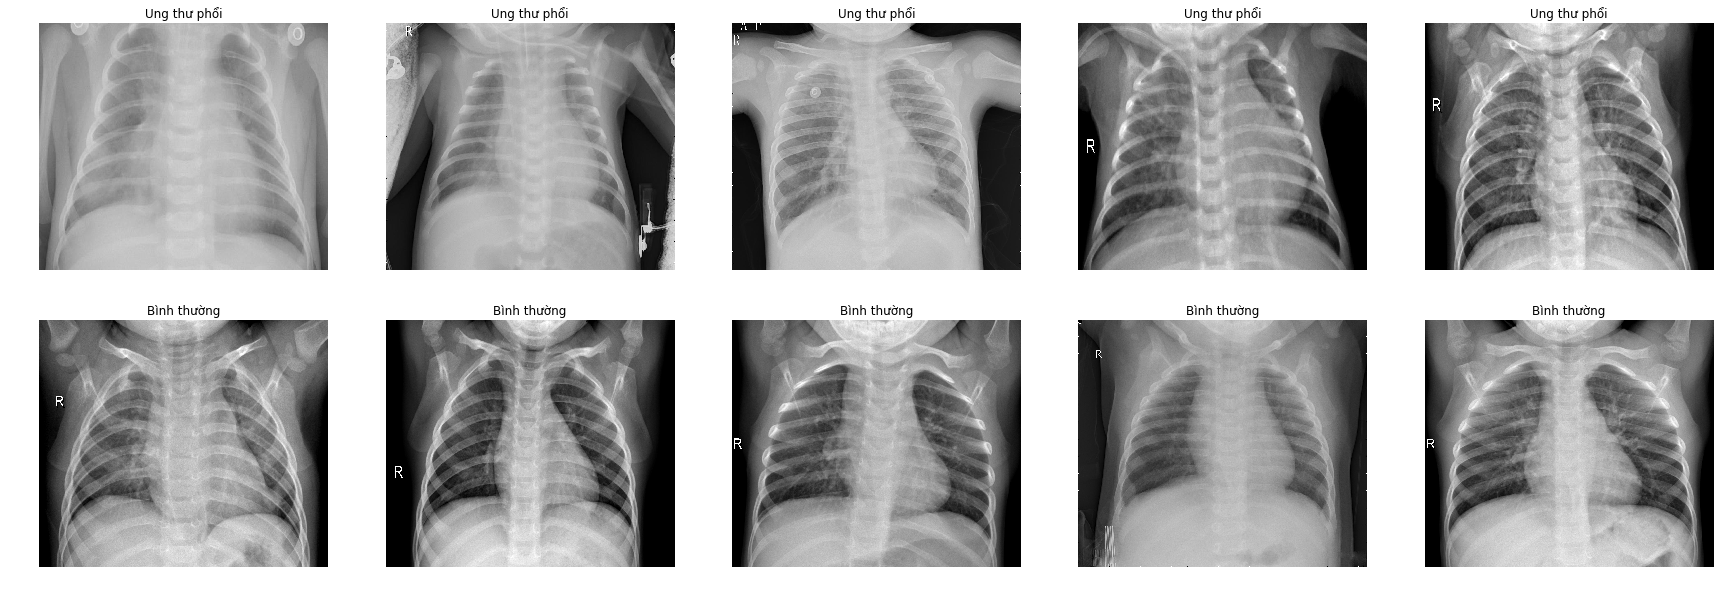
\includegraphics[width=0.95\linewidth,height=0.6\textheight]{show1.png}
	  \label{fig:writing-thesis}
	\end{figure}
 \end{column}
 \end{columns}
}
\section{} 
\frame{\frametitle {Kết luận}
\transblindshorizontal

 \begin{columns}
  \begin{column}{0.5\textwidth}
  \begin{small}
  \textbf{Đã làm được:}
\begin{itemize}
		\item Ứng dụng quy trình khai phá dữ liệu và rút trích các tri thức giá trị của dữ liệu đối với 3 dạng bài toán: Regression, Classification và Clustering.
		\item Thực hiện Model Tuning để cải thiện độ chính xác mô hình. 
		\item Thực hiện đánh giá mô hình qua nhiều phương pháp.
		\item Xây dựng Data Story một cách mạch lạc và trực quan.
\end{itemize} 
\end{small}
 \end{column}
  \begin{column}{0.5\textwidth}
     \setlength{\topsep}{0pt}
   \setlength{\partopsep}{0pt}
  \begin{small}
  \textbf{Chưa làm được:}
\begin{itemize}
		\item Độ chính xác mô hình Machine Learning chưa cao, do dữ liệu vẫn đang còn thiếu. \linebreak \linebreak \linebreak \linebreak \linebreak \linebreak \linebreak \linebreak \linebreak
		
\end{itemize} 
\end{small}
 \end{column}
 \end{columns}
}
\frame{\frametitle {}
\transblindshorizontal
  \begin{center}
	\textbf{\huge Cảm ơn quý thầy cô và các bạn đã lắng nghe!}
  \end{center}

}
\end{document}
%---------------------------------------------------------------------------------------------------------------------------------------------------------